\documentclass[style=upen, size=14pt]{powerdot}
\usepackage[round]{natbib}
\usepackage{bibentry}
\definecolor{arany}{RGB}{255,242,0}
\hypersetup{backref=page}
\hypersetup{
    colorlinks=true,
    linkcolor=cyan,
    citecolor=cyan,
    filecolor=magenta,      
    urlcolor=cyan}
% \pdsetup{trans=Split}
\usepackage{graphicx}
\usepackage{amsmath}
\DeclareMathOperator*{\argmax}{argmax}
\DeclareMathOperator*{\argmin}{argmin}
\DeclareMathOperator{\sign}{sign}
\usepackage{amssymb}
\usepackage{stmaryrd}
\usepackage[latin2]{inputenc}
%\usepackage[magyar]{babel}
%\usepackage{euler}
\usepackage{tikz}
\usetikzlibrary{matrix}
%\usepackage{tikz-qtree}
%\usepackage{tikz-dependency}
%\usepackage{linguex}
\usepackage{amsthm}
\usepackage{amsmath}
%\tikzset{every tree node/.style={align=center,anchor=north}}
%\usepackage{tabularx}
%\usepackage{threeparttable}
%\usepackage{color}
%\selectlanguage{english}
%\frenchspacing
\usepackage{algpseudocode}
\usepackage{algorithm} 
\newcommand{\nd}{\noindent}
\newcommand{\Val}{\mathop{\mathit{Val}}}
\newcommand{\gold}{\color{arany}}
%\usepackage{tikz}
%\usepackage{tikz-qtree}
%\newcommand{\qed}{\hfill\mbox{\raggedright \rule{.1in}{.1in}}}
\def\es{\mathbin\land}
\theoremstyle{definition}
\newtheorem*{definition}{Definition}
\newtheorem{axioma}{Axiom}
\newtheorem{tetel}{Theorem}
\newtheorem{prop}{Proposition}
\newtheorem{lemma}{Lemma}

\mathchardef\mhyphen="2D

\begin{document}

\title{Natural Language Processing\\~~\\Lecture 5\\Text classification and sequence tagging with classical methods}
% \author{}

\date{2021}
\maketitle

\section{Text classification}

\begin{slide}[toc=Tasks]{Text classification tasks}
  A text classification task is to assign the appropriate label from a given
  $C=\{c_1,\dots,c_n\}$ set of class/category labels to a $d$
  text/document.\bigskip

  Representative examples include
  \begin{itemize}
  \item \textbf{\gold Sentiment analysis}: classify according to the sentiment
    expressed by the document. Label set examples:
    \begin{itemize}
    \item  $\{$positive, negative$\}$,
    \item  $\{$positive, negative, ambigous$\}$, 
    \item $\{$admiration, amusement, annoyance, approval, \dots, sadness,
      surprise$\}$.\footnote{The example is based on the 27 emotions of the
        \href{https://arxiv.org/abs/2005.00547}{GoEmotions dataset}.}
    \end{itemize}
  \end{itemize}
\end{slide}

\begin{slide}[toc=]{Text classification tasks cont.}
  \begin{itemize}
  \item \textbf{\gold SPAM detection}: binary classification to decide whether
    a message is unsolicited.
  \item \textbf{\gold Authorship detection}: who wrote a text from a specified set of authors.
  \item \textbf{\gold Author characteristics detection}: was the author male or
    female, what was their age etc.
  \item \textbf{\gold Subject/topic detection}: to which subject/topic a
    document belongs to in a predefined list, e.g., in the Library of Congress Classification system
    $\{$medicine, agriculture, science, fine arts, \dots $\}$
  \item \textbf{\gold Genre detection}: determine the genre of a text, e.g.,
    assign a label from the set $\{$scifi, adventure, love story, mystery,
    historical, western$\}$.
    % \footnote{Labels from the paper
    %   \href{https://www.aclweb.org/anthology/C18-1167.pdf}{Genre Identification
    %     and the Compositional Effect of Genre in Literature}}
  \end{itemize}
 \end{slide}

 \begin{slide}[toc=Methods]{Methods}
   \begin{itemize}
   \item \textbf{\gold Manually designed rule-based systems}: e.g., using
     carefully designed lists of words positively or negatively correlated with
     the classes.
     
     These systems can reach good performance, but require a lot of manual work
     and are difficult to maintain and adapt.
   \item \textbf{\gold Machine learning methods}: Models learnt on a supervised
     data set containing labeled documents:
     $\{\langle d_i, c_i \rangle\}_{i\in \{1, \dots, N\}}$.

     Methods range from linear machine learning methods such as logistic
     regression to deep neural networks.
   \end{itemize}
 \end{slide}

 \begin{slide}[toc=Bag of words]{Bag of words (BOW) representation}
   Many machine learning-based classification methods require their input to be
   represented as fixed-length numerical  vectors. For texts with varying
   lengths, a common approach is use a bag of words representation:
   \begin{itemize}
   \item Tokenize the input texts using a $V=\{w_1,\dots,w_N\}$ vocabulary of
     word types, and
   \item represent them as $|V|=N$-dimensional vectors of word counts, i.e., for
     a $d$ document $BOW_V(d)=\langle c_{1,d}, \dots, c_{N,d}\rangle$, where each $c_{i,d}$
     is the count of $w_i$ in $d$.
   \end{itemize}
 \end{slide}

 
 \begin{slide}[toc=]{Bag of words representation cont.}
   A simple example:\smallskip
   
   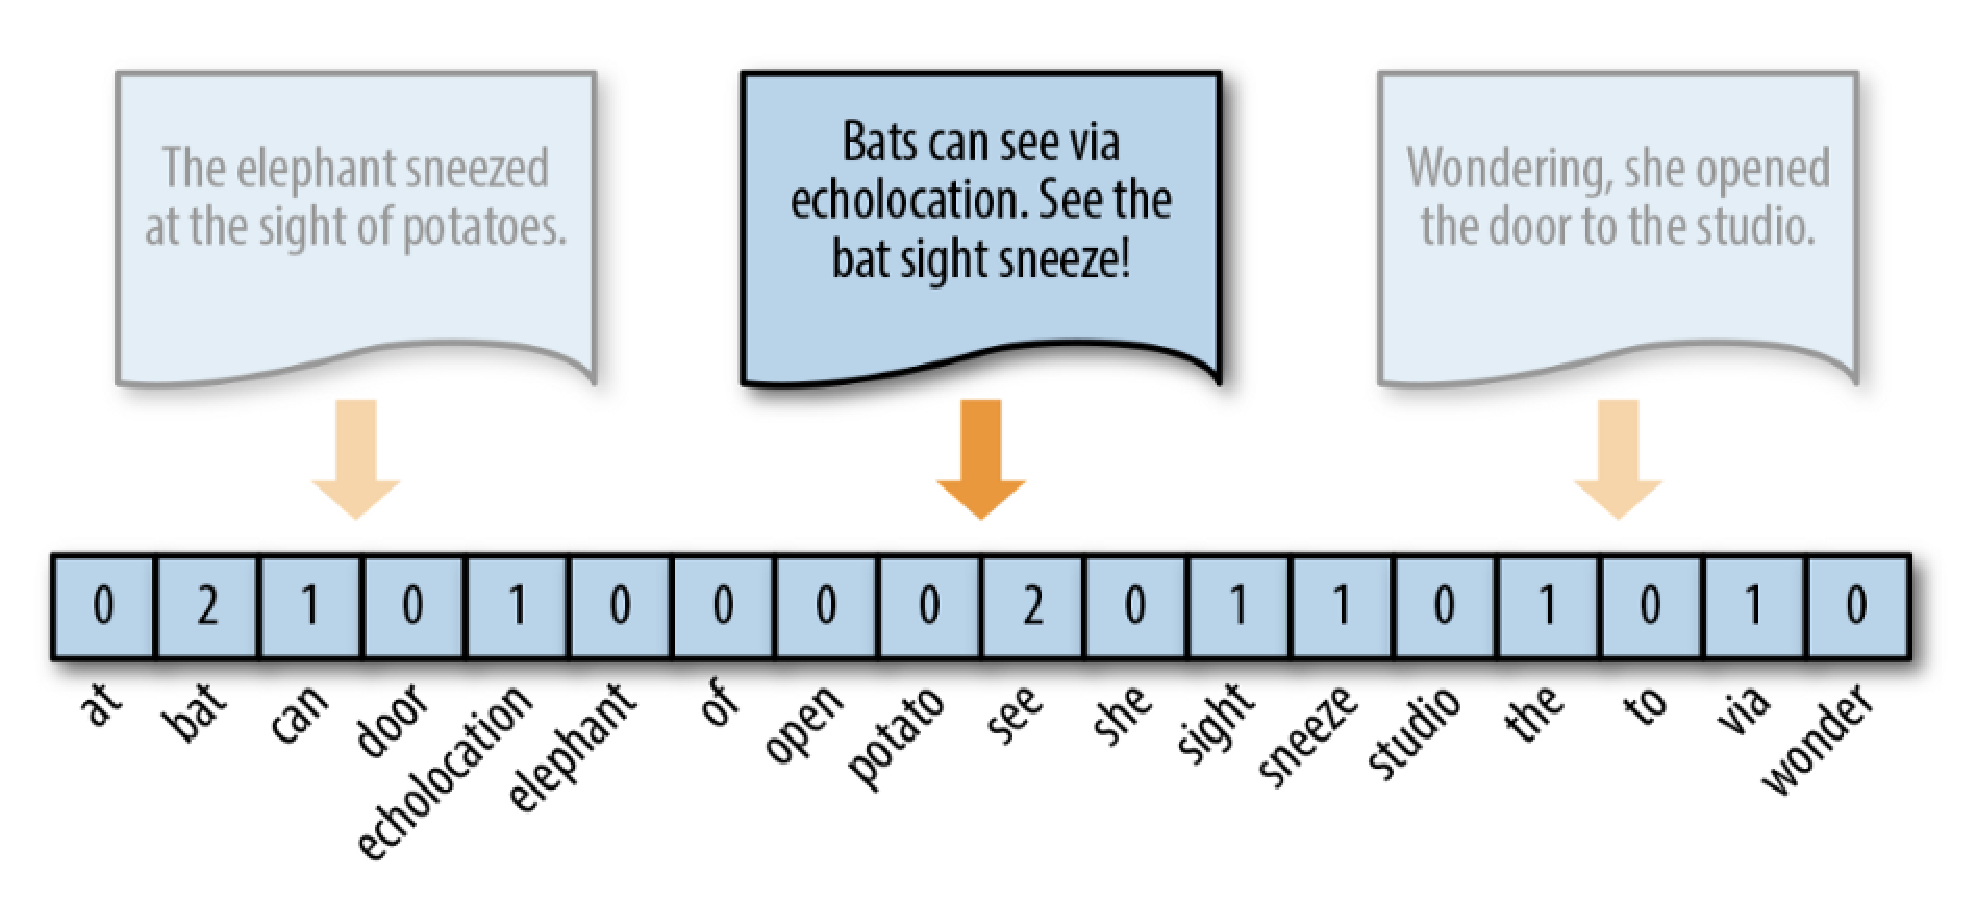
\includegraphics[width=1.0\textwidth]{figures/bow.eps}

   \begin{center}
     \footnotesize{(Figure from \href{https://towardsdatascience.com/from-word-embeddings-to-pretrained-language-models-a-new-age-in-nlp-part-1-7ed0c7f3dfc5}{From Word Embeddings to Pretrained Language Models}.)}     
   \end{center}
 \end{slide}

 \begin{slide}[toc=]{Bag of words refinements}
   The basic BOW representation can be refined in several ways, perhaps the
   three most important are
   \begin{itemize}
   \item omitting \emph{\gold stopword} (non-informative word) counts from the
     BOW vectors. What counts as stopword is task and domain dependent, but it
     is common to consider (some) function words, e.g. determiners to be
     stopwords;
   \item adding some word sequence counts to the BOW representations, e.g.,
     \emph{\gold bigram or trigram counts};
   \item weight words according to their informativity: the most widespread
     method is weighting according to \emph{\gold term frequency} and
     \emph{\gold inverse document frequency (TF-IDF)}.
   \end{itemize}
 \end{slide}


 \begin{slide}[toc=TF-IDF]{TF-IDF schemes}
   The basic assumption of TF-IDF weighting schemes is that words that occur in
   a large fraction of the training documents are not so informative as words
   occurring only in a few. TF-IDF vectors, accordingly discount word counts
   (``term frequencies'') by document frequencies. A simple but widespread
   variant:
   $$TF{\text -}IDF(d)=\langle tf_{1,d}\cdot idf_1, \dots, tf_{N,d}\cdot idf_N\rangle$$
   where $tf_{i,d}$ is simply the count of $w_i$ in $d$, while
   $$
   idf_i = \log\frac{\mathrm{\# of~~all~~documents}}{\mathrm{\# of~~documents~~containing}~~w_i  }
   $$
 \end{slide}

 \begin{slide}[toc=]{Binary bag of words}
   An interesting simplification of the BOW representation is to indicate only
   the presence or absence of words:

   $$BOW_{bin}(d)=\sign(BOW(d))$$

   where the application of the $\sign$ function is elementwise, i.e.,

   $$BOW_{bin}(d)=\langle \sign(c_{1,d}), \dots, \sign(c_{N,d})\rangle.$$
   
   It turned out that these simpler and less memory consuming representations
   can be used instead of normal BOW vectors in many settings without noticeable
   performance difference.
 \end{slide}

 \begin{slide}[toc=Naive Bayes]{Naive Bayes classifier with BOW}
   In its simplest form, the Naive Bayes (NB) classifier is a generative model
   modeling the joint distribution of $\mathbf{x}$ observation feature vectors
   and their $c$ class labels as
   $$
   P(\mathbf{x}, c) = P(c)\prod_{i=1}^D P(x_i~\vert~c).
   $$
   The model is ``naive'', because it is based on the \emph{conditional
     independence assumption} that given the class label, all observed features
   are independent of each other.
 \end{slide}

 \begin{slide}[toc=]{Naive Bayes classifier with BOW cont.}
   NB models can be precisely described by specifying
   \begin{itemize}
   \item the class label categorical distribution $P(c)$, and the
   \item the $P(x_i~\vert~ c_j)$ distributions for each $x_i$ observation
     feature and $c_j$ label.
   \end{itemize}
   $P(c)$ is always a categorical (Bernoulli or ``multinoulli'') distribution,
   while the choice of $P(x_i~\vert~ c_j)$ distributions depends on the type of
   $x_i$; for continuous $x_i$-s it can be any continuous distribution,
   Gaussian being a common choice.
 \end{slide}

 \begin{slide}[toc=]{Naive Bayes classifier with BOW cont.}
   The NB model can be adapted to text classification by applying the NB
   assumption to individual tokens: each token is assumed to be chosen
   independently from others according to a categorical conditional distribution
   $P(w ~|~ c)$. If $\mathbf{x}$ is a BOW vector and $c$ is a class label this
   means
   \begin{small}
   $$
   P(\mathbf{x}, c) = P(c) \prod_{i=1}^{|V|}P(w_i~\vert~c)^{x_i}.
   $$
   \end{small}
     Taking the logarithm of both sides for numerical stability reasons:
   \begin{small}
   $$
   \log P(\mathbf{x}, c) = \log P(c) + \sum_{i=1}^{|V|}x_i \log P(w_i~\vert~c).
   $$
   \end{small}
 \end{slide}

 \begin{slide}[toc=]{Naive Bayes classifier with BOW cont.}
   This means that given an $\mathbf{x}$ BOW vector and a vector
   $$\theta_c=\langle \log P(w_1~\vert~c),\dots,\log P(w_{|V|}~\vert~c) \rangle$$
   of conditional log probabilities of words for a $c$ class,
   $$\log P(\mathbf{x}, c) = \log P(c) +  \theta_c \cdot \mathbf{x},$$
   i.e., the log probability of $(\mathbf{x}, c)$ is a simple linear function
   for each $c_i$. Prediction of the most likely class for a $d$ document is also
   very simple:
   $$
   \hat c = \argmax_{c\in C}(\log P(c) + \theta_{c}  \cdot BOW(d) )
   $$
 \end{slide}

 \begin{slide}[toc=]{Naive Bayes classifier with BOW cont.}
   The MLE of the model parameters can be based on simple counts:
   $$
   P(c) \approx \frac{\# \mathrm{of}~~c~~\mathrm{documents}}{ \# \mathrm{of~~all~~documents}},
   $$
   $$
   P(w~|~c) \approx \frac{\# w~~\mathrm{occurrences~~in}~~c~~\mathrm{documents}}{\# of~~\mathrm{words~~in}~~c~~\mathrm{documents}}.
   $$\smallskip
   
   As we are basically working with per-class (unigram) language models, data
   sparsity presents problems again.
 \end{slide}

 \begin{slide}[toc=]{Naive Bayes classifier with BOW cont.}
   Most radically, if a word $w\in V$ does not occur in any $c$-class documents
   then the corpus-based MLE for $P(w~|~c)=0$ and, therefore, for any document
   with $\mathbf{x}$ BOW vector containing a non-zero count for  $w$
   $$
   P(\mathbf{x}, c) = P(c) \prod_{i=1}^{|V|}P(w_i~\vert~c)^{x_i}=0,
   $$
   regardless of any other word they contain.

   The solution is, again, using appropriate smoothing methods, e.g., add-one
   smoothing.
 \end{slide}

 \begin{slide}[toc=]{Naive Bayes limitations}
   Although BOW-based NB models are fairly simple to estimate and use for
   prediction, and can perform acceptably, there are some negatives:
   \begin{itemize}
   \item The NB conditional independence assumption is rather unrealistic and
     leads to misleading probability predictions with basic BOW;
   \item the NB assumption makes -- at least in theory -- the use of $N$-gram
     based BOW feature vectors even more questionable than unigrams;
   \item using a full generative model for a discriminative task typically has
     some performance penalties.
   \end{itemize}
 \end{slide}

 \begin{slide}[toc=Discriminative methods]{Discriminative linear methods}
   The most important alternative within the domain of classical learning
   algorithms is to use one of the well known \emph{discriminative methods} with
   BOW vectors:
   \begin{itemize}
   \item a perceptron variant,
   \item logistic regression, or  
   \item SVM.
   \end{itemize}
   These models do not assume conditional independence and therefore have no
   problem with using refined (e.g. $N$-gram based) BOW representations as input.
 \end{slide}

 \section{Sequence tagging}

 \begin{slide}[toc=Tagging tasks in NLP]{Sequence tagging in NLP}
   The sequence tagging task in general is to tag each element of a variable
   length input sequence with one of the labels in a given finite $T$ tag set.
   In NLP, the input sequence is typically a $\langle w_1,\dots,w_n \rangle$
   sequence of \emph{tokens}. Hence the alternative name
   \emph{\gold token classification}.\bigskip

   Some tasks in the traditional NLP pipeline are explicitly sequence tagging
   tasks, e.g. POS-tagging and morphological tagging. Others, like NP-chunking,
   NER or keyword identification can be transformed into a sequence tagging task
   with a simple trick.
 \end{slide}

 \begin{slide}[toc=IOB tagging]{IOB tagging}
   These tasks are ostensibly span-finding and span-tagging tasks: the goal is
   to find token spans belonging the certain categories.

   E.g., in the case of (minimal) noun phrase (NP) chunking:
   \begin{center}
     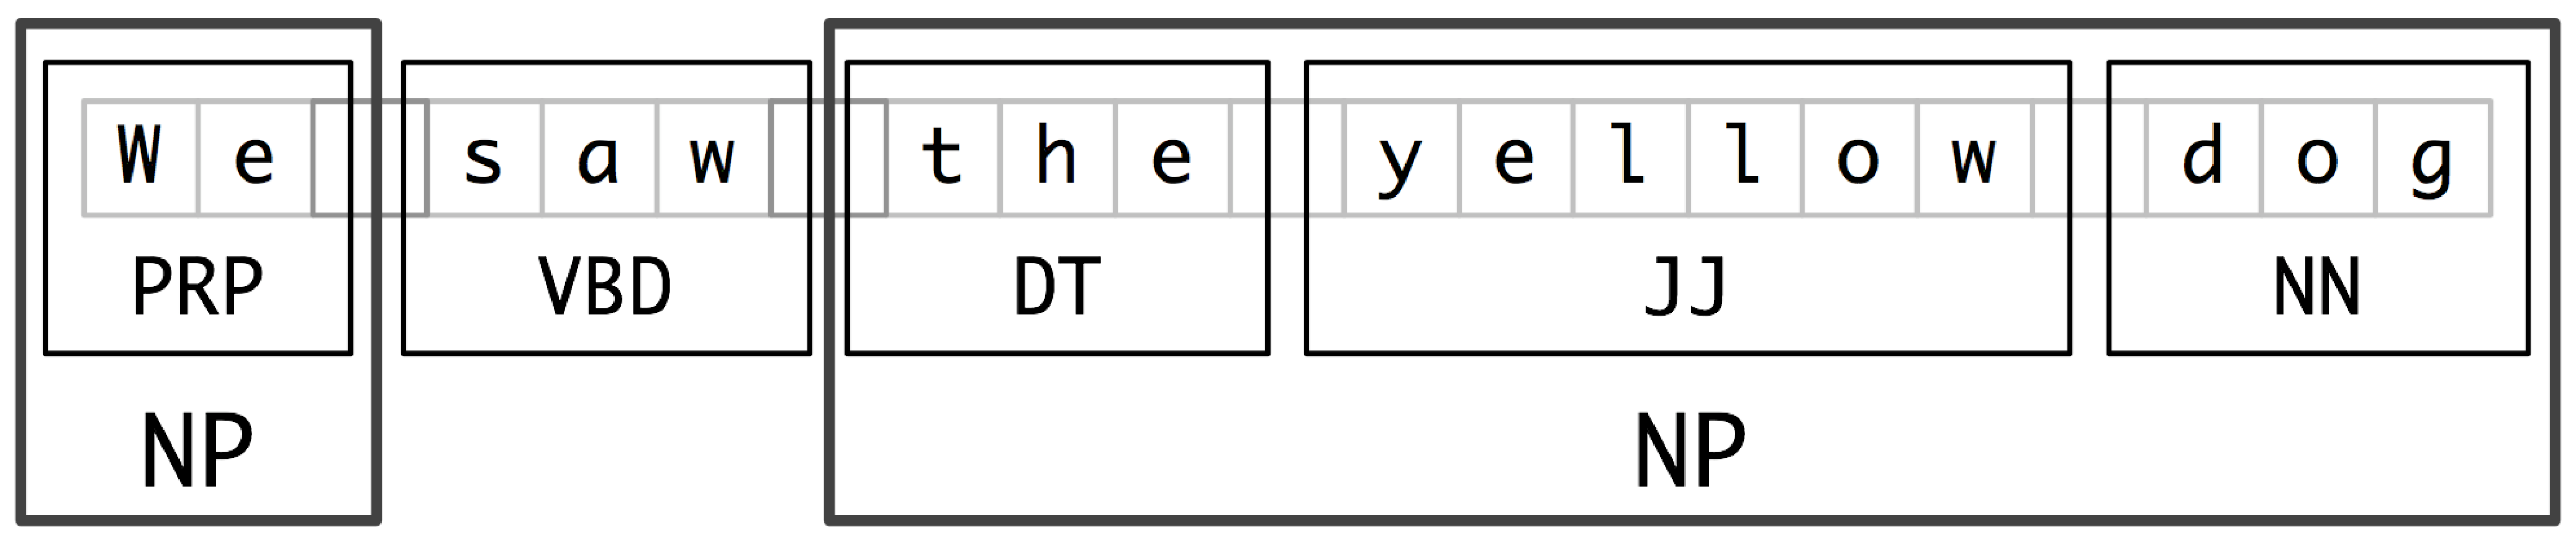
\includegraphics[width=1.0\textwidth]{figures/iob1.eps}
   \footnotesize(Figure from the \href{http://www.nltk.org/book/ch07.html}{NLTK book}.)
 \end{center}
 \end{slide}

 \begin{slide}[toc=]{IOB tagging cont.} 
   The IOB trick is to reformulate the span identification/tagging task as a
   sequence tagging task. If there are $T_1,\dots,T_N$ span
   types to be identified, then we introduce three types of token-level tags:
   \begin{itemize}
     \item a $B$ (beginning) tag for all span types:
       $B\mhyphen{}T_1,\dots,B\mhyphen{}T_N$ indicating the first token of a
       span of a given type;
   \item an $I$ (inside) tag for all span types
       $I\mhyphen{}T_1,\dots,I\mhyphen{}T_N$; indicating that a token is inside
       (as second or later element) a span, and, finally,
   \item a unique $O$ tag for tokens that do not belong to any span type to be
     found.
   \end{itemize}
 \end{slide}
 
 \begin{slide}[toc=]{IOB tagging cont.}
   Using these tags the span identification task becomes a sequence tagging
   task.
   
   \begin{center}
     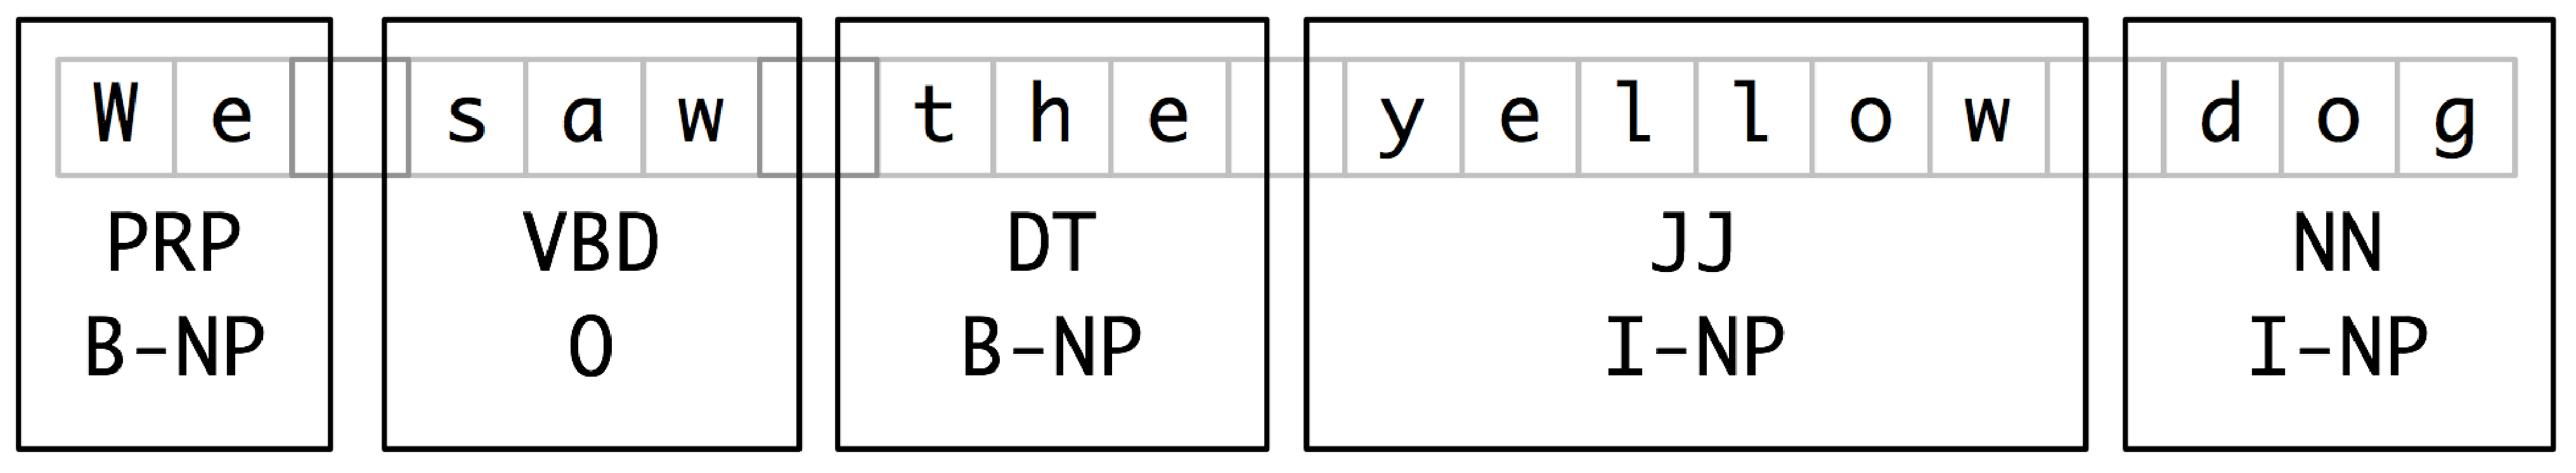
\includegraphics[width=1.0\textwidth]{figures/iob2.eps}
     \footnotesize(Figure from the \href{http://www.nltk.org/book/ch07.html}{NLTK book}.)
    \end{center}
    
    Other schemes exist along IOB (BIO), the most popular being BIOES, which
    introduces $E\mhyphen{}T_i$ \emph{end} tags, as well as $S\mhyphen{}T_i$
    tags for single-token spans.
    % Although the IOB (BIO) scheme is the most well known, others are in use as
    % well.
    % e.g., if one introduces $E-T_i$ \emph{end} tags, then a unique $I$
    % \textit{inside} tag is enough for unambiguous tagging.
  \end{slide}

  \begin{slide}[toc=Challenges]{Sequence tagging challenges}
    The main challenge of sequence tagging is the complicated interdependence
    between the tag of an element and the features of the other elements
    \emph{including their tags}: in the case of most NLP tagging tasks, the
    tags are \emph{\gold strongly context dependent}.\bigskip

    Another important problem is feature engineering: which features of the
    sequence elements are relevant for tagging? If out of vocabulary words are
    to be handled properly then at least some of the features should probably be
    based on the word's surface form, e.g. on its capitalization, suffix etc.    
  \end{slide}
  
  \begin{slide}[toc=Supervised methods]{Supervised methods for sequence tagging}
    These methods assume that a
    $$D=\{\langle \mathbf{x_1},\mathbf{y_1} \rangle,\dots, \langle \mathbf{x_N},\mathbf{y_N} \rangle\}$$
    supervised dataset is available, in which each
    $\langle \mathbf{x}_i, \mathbf{y}_i \rangle$ pair consists of an
    $\langle x_1^i,\dots,x_{n_i}^i\rangle$ sequence to be tagged and the
    corresponding $\langle y_1^i,\dots,y_{n_i}^i\rangle$ correct tag sequence.\bigskip

    The methods we will discuss are all \emph{probabilistic}: they model either
    the $ P(\mathbf{X}, \mathbf{Y}) $ joint distribution (generative model) or
    the $ P(\mathbf{Y}~|~\mathbf{X}) $ conditional distribution (discriminative
    model).
  \end{slide}

  \begin{slide}[toc=HMMs]{Hidden Markov models (HMMs)}
    HMMs are \emph{generative models} of the $P(\mathbf{X}, \mathbf{Y})$
    distribution based on the assumption that the elements of the \emph{\gold
      observable} $\mathbf{x}$ sequences actually depend on the positionally
    corresponding \emph{\gold hidden} elements of the $\mathbf{y}$ sequences,
    which, in turn, are distributed according to a Markov model. The conditional
    independence assumptions collectively follow this graphical model:
    \begin{center}
      \begin{tikzpicture}[ampersand replacement=\&]
        \matrix[matrix of math nodes,column sep=2em,row sep=3em] (m) {
          Y_1 \& Y_2 \& Y_3 \& \cdots \& Y_{n}\\
          X_1 \& X_2 \& X_3 \& \dots \& X_n\\
        };
        \foreach \X in {1,2,3,4}
        {\draw[-latex] (m-1-\X) -- (m-1-\the\numexpr\X+1) ;
          \ifnum\X=4
          \draw[-latex] (m-1-5) -- (m-2-5) ;
          \else
          \draw[-latex] (m-1-\X) -- (m-2-\X);
          \fi}
        % \draw[dashed] ([yshift=1ex]m.east) -- ([yshift=1ex]m.east-|m-1-1.east);
      \end{tikzpicture}
    \end{center}
  \end{slide}

  \begin{slide}[toc=]{Hidden Markov models cont.}
    Because of the Markov model assumption regarding the $Y$s, there is an
    $A$ matrix specifying all tag \emph{\gold transition probabilities}, so
    that for any appropriate $k, i, j$,
    $$
    P(Y_k=y_j ~|~Y_{k-1}=y_i) = a_{i j}.
    $$
    HMMs also assume that the $P(X~|~Y)$ \emph{\gold emission probabilities} are
    position-independent: there is also a $B$ matrix so that for any
    $k, i, j$,
    $$
    P(X_k= x_j ~|~Y_{k}= y_i) = b_{i j}.
    $$
  \end{slide}

  \begin{slide}[toc=]{Hidden Markov models cont.}
    Assuming, finally, a $\Pi$ vector containing the start probabilities
    for each possible $y_i$ tag:
    $$
    P(Y_1 = y_i) = \pi_i,
    $$
    the probability of a concrete
    $\langle \mathbf{x}, \mathbf{y} \rangle =\langle \langle
    x_{l_1},\dots,x_{l_n} \rangle, \langle y_{m_1},\dots,y_{m_n} \rangle
    \rangle$ pair can be calculated as
    $$
    P(\mathbf{x}, \mathbf{y}) = \pi_{m_1} b_{m_1 l_1}
    \prod_{i=2}^na_{m_{i-1} m_i}b_{m_i l_i}.
    $$
  \end{slide}

  \begin{slide}[toc=]{Hidden Markov models cont.} The MLE of the probabilities
    in $A, B$ and $\Pi$ can be calculated simply by counting. If the training
    dataset contains $N$ sequences then
    \begin{gather*} \pi_i = \frac{C(\mathrm{first~~element~~is~~}
        y_i)}{N}\\ a_{ij} = \frac{C(\langle y_i,y_j\rangle)}{\sum_kC(\langle
        y_i,y_k\rangle)}\\ b_{ij} = \frac{C(y_i \mathrm{~~emits~~} x_j)}{C(y_i)}
    \end{gather*}
    Similarly to other counting based MLE methods, smoothing might be necessary
    in case of sparse data.
  \end{slide}

  \begin{slide}[toc=Viterbi]{The Viterbi algorithm}
    Given a trained HMM with $\pi, A, B$ parameters, and an $\mathbf{x}$
    input sequence of length $n$, we want to determine the most probable corresponding
    $\mathbf{y}$ sequence of tags, i.e. find
    $$
    \argmax_{\mathbf{y}\in Y^n} P(\mathbf{y} ~|~ \mathbf{x}, \Pi, A, B),
    $$
    which equals
    $$
    \argmax_{\mathbf{y}\in Y^n} P(\mathbf{x}, \mathbf{y} ~|~ \Pi, A, B).
    $$
    An exhaustive search is unfeasible because there are $|Y|^n$ alternative tag
    sequences.
  \end{slide}
  
  \begin{slide}[toc=]{The Viterbi algorithm cont.}
    Fortunately, the HMM conditional independence assumptions have the following
    consequence: If we know, for all $y_i\in Y$, the values
    $$
    \mathbf{y}^{n-1}_i = \argmax_{\mathbf{y}\in Y^{n-1}~\wedge~\mathbf{y}[n-1] = y_i}
    P(\mathbf{x}[1:n-1], \mathbf{y} ~|~ \Pi, A, B),
    $$
    (i.e. the most probable $n-1$-long tag sequences ending in $y_i$),
    then the most probable $\mathbf{y}$ can be computed by comparing only
    $|Y|^2$ continuations:
    \begin{gather*}
      \mathbf{y} = \argmax_{\mathbf{y}\in \{\langle \mathbf{y}_i^{n-1},~y \rangle ~|~ i \in 1\dots |Y|~\wedge~ y \in Y\}} P(\mathbf{x}, \mathbf{y} ~|~ \Pi, A, B).
    \end{gather*}
    % i.e., we need to search only among the $|Y|^2$ possible continuations of the
    % $\mathbf{y}^{n-1}_i$ sequences.
  \end{slide}

  \begin{slide}[toc=]{The Viterbi algorithm cont.}
    This suggests the following algorithm (named after Andrew Viterbi, who
    published a variant in 1967):\bigskip

	\small
    \begin{algorithmic}[1]
	
      \ForAll{$i\in 1\dots |Y|$}
      \State $\mathbf{y}_i^1 \leftarrow \langle y_i \rangle$
      \EndFor
      \ForAll{$t\in 2\dots n-1$}
      \ForAll{$i\in 1\dots |Y|$}
      \State{
        $$\mathbf{y}_i^t \leftarrow  \argmax_{\mathbf{y}\in \{\langle \mathbf{y}_k^{t-1}, y_i \rangle ~|~         k \in 1\dots |Y|\}} P(\mathbf{x}[1:t], \mathbf{y} ~|~ \Pi, A, B)
        $$}
      \EndFor
      \EndFor
      \State{\Return{$\argmax_{\mathbf{y}\in \{\langle \mathbf{y}_i^{n-1},~y \rangle ~|~ i \in 1\dots |Y|~\wedge~ y \in Y\}} P(\mathbf{x}, \mathbf{y} ~|~ \Pi, A, B)$}}
    \end{algorithmic}
  \end{slide}
  
  \begin{slide}[toc=]{The Viterbi algorithm cont.}
    The algorithm maintains an $|Y| \times \mathrm{length}(\mathbf{x})$ table.
    In the \emph{forward pass}, it
    \begin{enumerate}
      \item computes the probabilities of the $y_i^t$s x
      \item maintains backreferences to the most probable $\mathbf{y}^{t-1}$
    \end{enumerate}

    In the \emph{backward pass}, the most probable $y_i^n$ is
    selected and $\mathbf{y}$ is recovered by following the
    backreferences.

    \begin{center}
      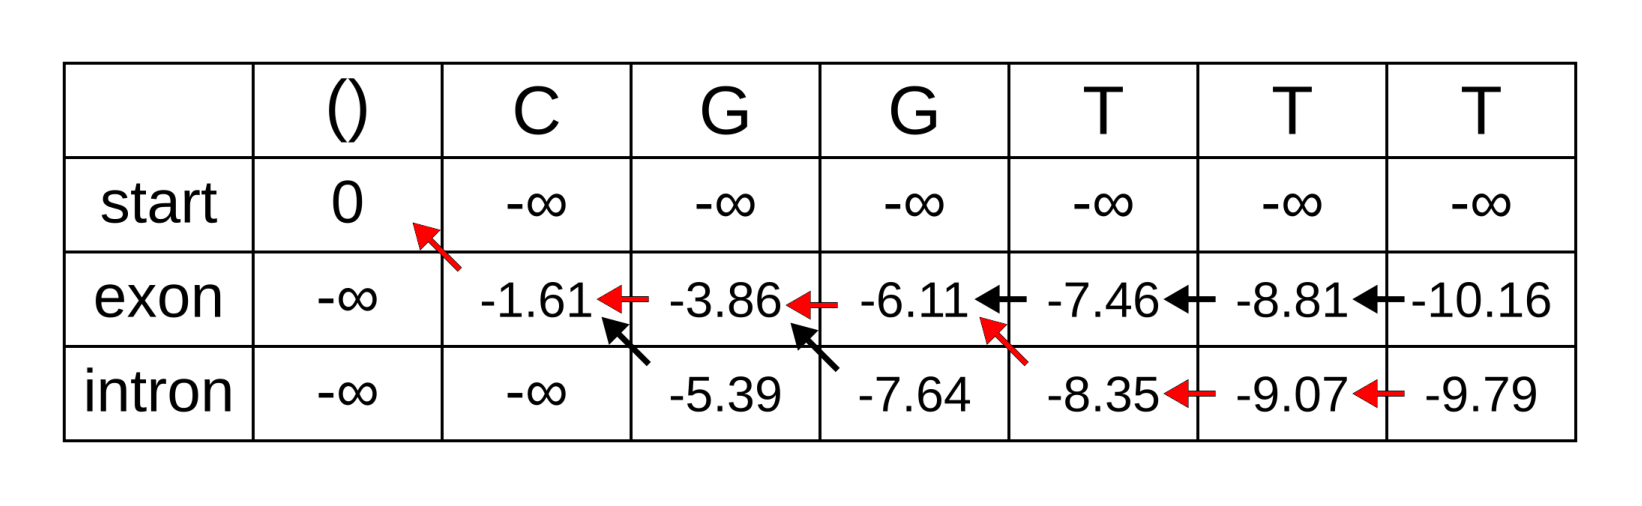
\includegraphics[width=0.8\textwidth]{figures/viterbi-5.eps}
      
      \footnotesize(Figure from the \href{https://cs.rice.edu/~ogilvie/comp571/viterbi-algorithm/}{Species and Gene Evolution} blog.)
    \end{center}
  \end{slide}
    
  \begin{slide}[toc=]{The Viterbi algorithm cont.}
    Viterbi is a \emph{\href{https://en.wikipedia.org/wiki/Dynamic_programming}{dynamic programming}} algorithm that, in stark contrast
    to an exhaustive search, has a time complexity of
    $\mathcal O(\mathrm{length}(\mathbf{x})|Y|^2)$.\medskip

    The table that tracks the partial $\mathbf{y}_i^t$ sequence elements and
    their probabilities only takes up
    $\mathcal{O}(\mathrm{length}(\mathbf{x})|Y|)$ space.\medskip


    Calculating the probabilities to be compared directly requires multiplying
    numbers very close to zero, so it is customary to work with log
    probabilities instead.\medskip %(and addition) instead.

    \begin{small}
      Note: the Viterbi algorithm is also known as the \emph{\href{http://www.inference.org.uk/itprnn/book.pdf}{min-sum}} algorithm. See \citet[p. 245]{mackay2003information}.
    \end{small}
  \end{slide}

  \begin{slide}[toc=Discriminative methods]{Discriminative methods}
    Similarly to the Naive Bayes sequence classifier, HMMs are generative
    models, modeling probabilities of the input as well as the labels, which is
    unnecessary in our setting. We can construct similarly structured but
    \emph{discriminative} models by ``reversing the arrows'' between input and
    labels and conditionalizing on $\mathbf{X}$:

    
    \begin{center}
      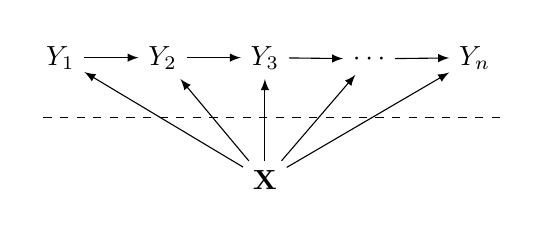
\begin{tikzpicture}[ampersand replacement=\&]
        \matrix[matrix of math nodes,column sep=2em,row sep=3em] (m) {
          Y_1 \& Y_2 \& Y_3 \& \cdots \& Y_{n}\\
           \&  \& \mathbf{X} \&  \& \\
        };
        \foreach \X in {1,2,3,4}
        {\draw[-latex] (m-1-\X) -- (m-1-\the\numexpr\X+1) ;
          \draw[-latex] (m-2-3) -- (m-1-\X) ;
        }
        \draw[-latex] (m-2-3) -- (m-1-5);
        \draw[dashed] ([yshift=0ex]m.east-|m-1-5.east) -- ([yshift=0ex]m.east-|m-1-1.west);
      \end{tikzpicture}
    \end{center}
  \end{slide}

  \begin{slide}[toc=MEMMs]{Maximum entropy Markov models (MEMMs)}
    According to the previous graphical model's assumptions,
    \begin{small}
      $$
      P(\mathbf{Y}~|~\mathbf{X}) = P(Y_1~|~ \mathbf{X})\prod_{m=2}^n P(Y_m|Y_{m-1}, \mathbf{X}).
      $$
    \end{small}%
    MEMMs further constrain this generic model by making $y_m$ conditionally
    independent of all observations other than $x_m$:
    \begin{small}
      $$
      P(\mathbf{Y}~|~\mathbf{X}) = P(Y_1~|~X_1)\prod_{m=2}^n P(Y_m|Y_{m-1},X_m).
      $$
  \end{small}
  \end{slide}

  \begin{slide}[toc=MEMMs]{Maximum entropy Markov models (MEMMs)}
    The individual $P(Y_m|Y_{m-1},X_m)$ probabilities are modelled
    analogously to \emph{multinomial logistic regression} with the
    softmax function:
    \begin{small}
      $$
      P(Y_m = y_i|Y_{m-1}=y_k,\mathbf{x})=\frac{\exp (\mathbf{w}_i \cdot \mathbf{f}(y_k,
        \mathbf{x}, m))}{\sum_{j=1}^{|Y|}\exp (\mathbf{w}_j \cdot \mathbf{f}(y_k,
        \mathbf{x}, m))},
      $$
      where $\mathbf{f}(\cdot)$ is a feature vector producing function, and each
      $\mathbf{w}_i$ is a weight vector for the $y_i\in Y$ label. (Note how
      we replaced $x_m$ with $\mathbf{f}(y_{m-1}, \mathbf{x}, m)$; see next
      slide why!)\bigskip
    \end{small}

    The name MEMM comes from the fact that in NLP, multinomial logistic
    regression is better known by the name \emph{maximum entropy}.
  \end{slide}

  \begin{slide}[toc=Feature functions]{Feature functions}
    MEMM feature functions were traditionally designed by field experts. In NLP
    it is customary to condition only on \emph{local features} of the element to
    be tagged and consider only a \emph{context window}. E.g., for POS tagging,
    $\mathbf{f}(y_{m-1},\mathbf{x}, m)$ would include the features:
    \begin{itemize}
    \item Elements in a context window around $x_m$, e.g.
      $\langle x_{m-1}, x_{m}, x_{m+1} \rangle$,
    \item suffixes (of a fixed length) of the context window's elements,
    \item prefixes (of a fixed length) of the context window's elements,
    \item capitalization information of the context window's elements.
    \end{itemize}
    
    % WARNING: A typical feature template like the above can actually produce
    % \emph{thousands of features} because the categoricals have to be one-hot
    % encoded. In addition to performance implications this also has consequences
    % for data sparsity: smoothing becomes very important.
    
  \end{slide}

  \begin{slide}[toc=CRFs]{Conditional Random Fields (CRFs)}
    Although MEMMs are more flexible than HMMs (e.g., tags can depend on other
    features of the context than the previous tag), they also have important
    limitations.\bigskip

    Perhaps the most important is that the label probabilities are \emph{locally
      normalized}: $\sum_{y\in Y}P(y~|y_{m-1}, \mathbf{x}, m)=1$ independently
    of how ``familiar'' a context is to the model, and, therefore, the model
    cannot express a general low confidence about the labels in a given context.
    This leads to the so-called \emph{\href{https://awni.github.io/label-bias/}{label bias}} problem: the model prefers
    labels with low entropy next label distributions, even if they have low
    confidence. Linear-chain CRF models were designed to address these problems.
  \end{slide}

  \begin{slide}[toc=]{Label bias}
    Label bias in action:
    \begin{small}
      \begin{itemize}
        \item A POS tagger receives the sentence ``\textit{cat sat}''
        \item The output is \texttt{ARTICLE VERB}, because of the
          posterior distribution of \textit{cat} at \texttt{<S>} with
          \textbf{local} normalization (left)
        \item The unnormalized (log) probabilities (right) reveal that that
          distribution is dwarfed by the other options and \texttt{NOUN VERB}
          is more probable \textbf{globally}.
      \end{itemize}
    \end{small}

    \begin{center}
      \begin{minipage}{0.45\textwidth}
        \begin{center}
        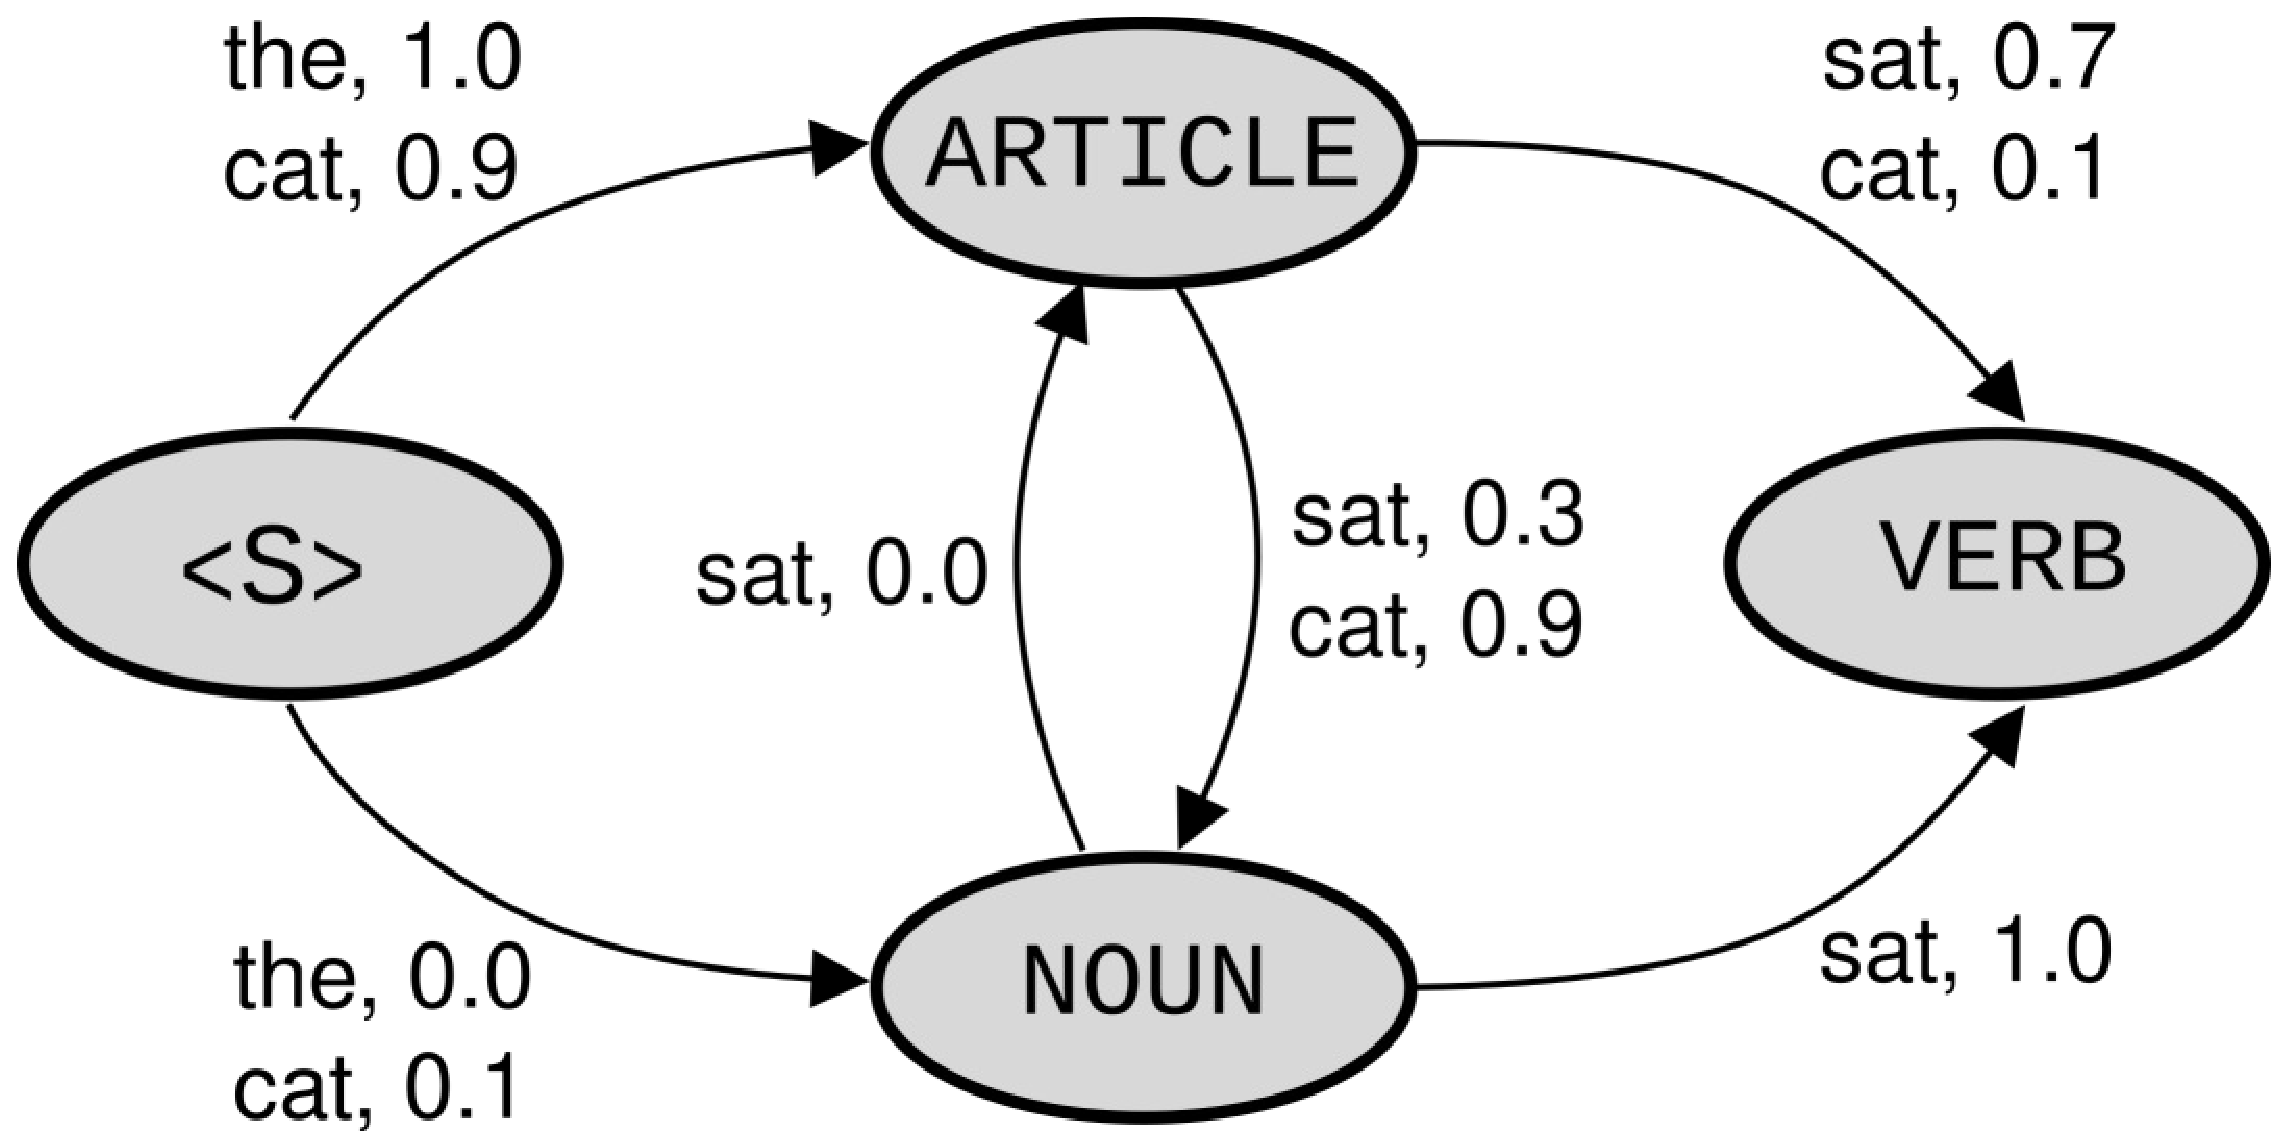
\includegraphics[width=0.9\textwidth]{figures/memm_inference_normalized.eps}
        \end{center}
      \end{minipage}\hfill
      \begin{minipage}{0.45\textwidth}
        \begin{center}
        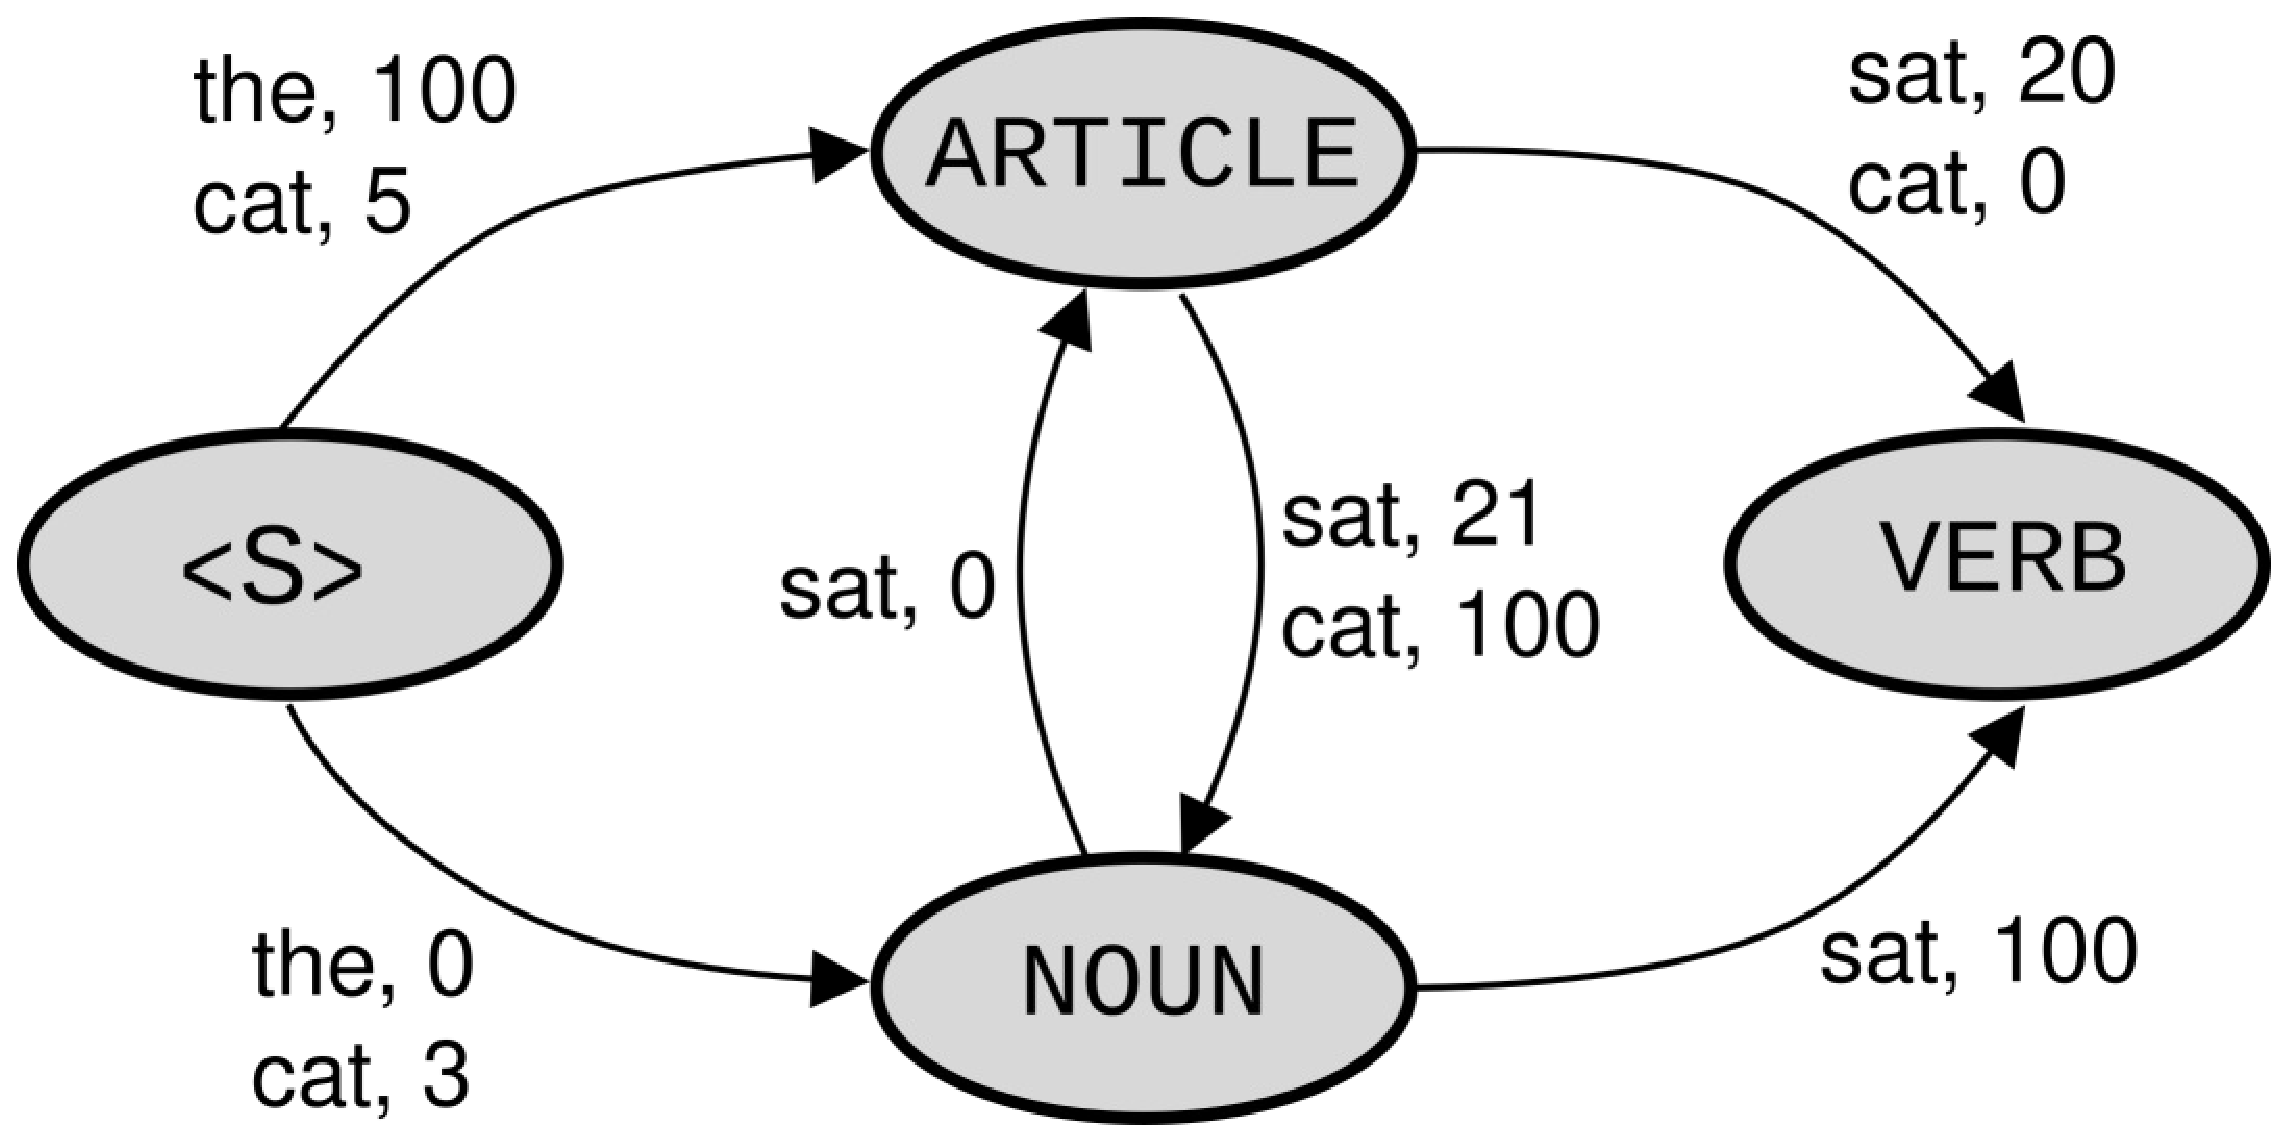
\includegraphics[width=0.9\textwidth]{figures/memm_inference_unnormalized.eps}
        \end{center}
      \end{minipage}

      \footnotesize(Figures from the \href{https://awni.github.io/label-bias/}{Awni Hannun -- Writing About Machine Learning} blog.)
    \end{center}
  \end{slide}

  \begin{slide}[toc=]{Conditional Random Fields cont.}
    Linear chain CRFs are discriminative models assuming the following
    \emph{undirected} structure:
    \begin{center}
      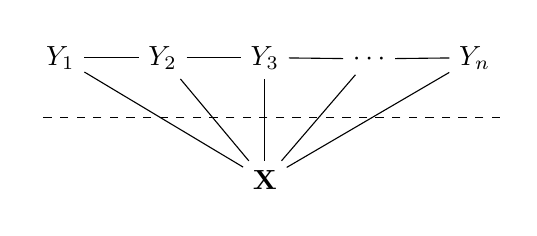
\begin{tikzpicture}[ampersand replacement=\&]
        \matrix[matrix of math nodes,column sep=2em,row sep=3em] (m) {
          Y_1 \& Y_2 \& Y_3 \& \cdots \& Y_{n}\\
           \&  \& \mathbf{X} \&  \& \\
        };
        \foreach \X in {1,2,3,4}
        {\draw (m-1-\X) -- (m-1-\the\numexpr\X+1) ;
          \draw  (m-2-3) -- (m-1-\X) ;
        }
        \draw (m-2-3) -- (m-1-5);
        \draw[dashed] ([yshift=0ex]m.east-|m-1-5.east) -- ([yshift=0ex]m.east-|m-1-1.west);
      \end{tikzpicture}
    \end{center}
    According to these assumptions,
    $$
    P(\mathbf{Y}~|~\mathbf{X}) = \frac{1}{Z(\mathbf{X})}\prod_{m=1}^{n-1} \phi_{m}(Y_m, Y_{m+1}, \mathbf{X}).
    $$
  \end{slide}

  \begin{slide}[toc=]{Conditional Random Fields cont.}
    Somewhat similarly to MEMMs, the $\phi_m(\cdot)$ potential functions are
    modeled linearly using a feature function and a corresponding weight vector:
    $$
    \phi_m(y_m, y_{m+1},\mathbf{x})={\exp (\mathbf{w} \cdot
      \mathbf{f}(y_m,y_{m+1}, \mathbf{x}, m))}.
    $$
    The crucial difference compared to MEMMs is that the normalization is \emph{global}:
    $$
    P(\mathbf{y}~|~\mathbf{x}) =
    \frac{\exp(\sum_{m=1}^{n-1}\mathbf{w}\cdot\mathbf{f}(y_m,y_{m+1}, \mathbf{x}, m))}
    {\sum_{\mathbf{y}'\in Y^n}\exp(\sum_{m=1}^{n-1}\mathbf{w}\cdot\mathbf{f}(y'_m,y'_{m+1}, \mathbf{x}, m))}.
    $$
    
  \end{slide}

  \begin{slide}[toc={Optimization and inference}]{Optimization and inference}
    Both MEMMs and linear chain CRFs can be optimized using standard convex
    optimization techniques, e.g., gradient descent, and, having trained a
    model, the most likely tag sequence for a given input can be efficiently
    found by using variants of the Viterbi algorithm.
  \end{slide}

  \begin{slide}{References}
    \bibliographystyle{plainnat}
    \nobibliography{nlp_course.bib}
    \begin{footnotesize}

      \bibentry{mackay2003information}.\medskip
      
    \end{footnotesize}
  \end{slide}

\end{document}



%%% Local Variables:
%%% mode: latex 
%%% TeX-master: t
%%% End:

% LocalWords:  Tokenization Discriminative discriminative
